\begin{tikzpicture}[x=1.4cm, y=1.0cm, >=stealth]

% ============================================================
% TITLE
% ============================================================
\node[font=\large\bfseries] at (4.5, 22.0)
  {The Geometry of Rational Approximation};

% ============================================================
% SECTION 1 — FAREY NUMBER LINE
%
% Vertical slots (top to bottom):
%   21.2  left sub-gap label
%   21.2  right sub-gap label
%   20.6  sub-gap arrows  ←——→ ←——→
%   20.0  NUMBER LINE
%   19.2  fraction labels a/b  (a+c)/(b+d)  c/d
%   18.2  full-gap arrow ←————————————→
%   17.6  full-gap label  c/d − a/b = 1/bd
% ============================================================

% Sub-gap labels (above the brackets)
\node[blue, font=\small, anchor=south] at (2.9, 20.65)
  {$\dfrac{a+c}{b+d}-\dfrac{a}{b}=\dfrac{1}{b(b+d)}$};
\node[blue, font=\small, anchor=south] at (6.1, 20.65)
  {$\dfrac{c}{d}-\dfrac{a+c}{b+d}=\dfrac{1}{d(b+d)}$};

% Sub-gap brackets
\draw[<->, blue, thick] (1.8, 20.6) -- (4.2, 20.6);
\draw[<->, blue, thick] (4.2, 20.6) -- (6.8, 20.6);

% Number line
\draw[thick] (0, 20.0) -- (9, 20.0);
\node[left=4pt]  at (0, 20.0) {$0$};
\node[right=4pt] at (9, 20.0) {$1$};

% Ticks on number line
\draw[thick]       (1.8, 20.13) -- (1.8, 19.87);
\draw[thick, blue] (4.2, 20.13) -- (4.2, 19.87);
\draw[thick]       (6.8, 20.13) -- (6.8, 19.87);

% Fraction labels below ticks
\node[below=6pt] at (1.8, 19.87)       {$\dfrac{a}{b}$};
\node[below=6pt, blue] at (4.2, 19.87) {$\dfrac{a+c}{b+d}$};
\node[below=6pt] at (6.8, 19.87)       {$\dfrac{c}{d}$};

% Full-gap arrow (below fraction labels — plenty of room)
\draw[<->] (1.8, 18.1) -- (6.8, 18.1);

% Full-gap label below arrow
\node[below=2pt] at (4.3, 18.1)
  {$\dfrac{c}{d}-\dfrac{a}{b}=\dfrac{1}{bd}$};

% ============================================================
% SECTION 2 — STERN-BROCOT HEADING
% ============================================================
\node[font=\bfseries] at (4.5, 16.6) {Stern--Brocot refinement};

% ============================================================
% SECTION 3 — STERN-BROCOT TREE
%   Level 0: y = 15.6
%   Level 1: y = 13.7
%   Level 2: y = 11.8
% ============================================================

% Level 0
\node at (0.7,  15.6) {$\dfrac{0}{1}$};
\node at (4.5,  15.6) {$\dfrac{1}{1}$};
\node at (8.3,  15.6) {$\dfrac{1}{0}$};

% Level 1
\node at (2.6,  13.7) {$\dfrac{1}{2}$};
\node at (6.4,  13.7) {$\dfrac{2}{1}$};

\draw (0.7,  15.3) -- (2.6,  14.15);
\draw (4.5,  15.3) -- (2.6,  14.15);
\draw (4.5,  15.3) -- (6.4,  14.15);
\draw (8.3,  15.3) -- (6.4,  14.15);

% Level 2
\node at (1.65, 11.8) {$\dfrac{1}{3}$};
\node at (3.55, 11.8) {$\dfrac{2}{3}$};
\node at (5.45, 11.8) {$\dfrac{3}{2}$};
\node at (7.35, 11.8) {$\dfrac{3}{1}$};

\draw (0.7,  15.3) -- (1.65, 12.25);
\draw (2.6,  13.3) -- (1.65, 12.25);

\draw (2.6,  13.3) -- (3.55, 12.25);
\draw (4.5,  15.3) -- (3.55, 12.25);

\draw (4.5,  15.3) -- (5.45, 12.25);
\draw (6.4,  13.3) -- (5.45, 12.25);

\draw (6.4,  13.3) -- (7.35, 12.25);
\draw (8.3,  15.3) -- (7.35, 12.25);

% ============================================================
% SECTION 4 — DIRICHLET APPROXIMATION
%
% x sits at horizontal position 5.15 on the number line (y=8.2).
% Circles centred exactly on x in the space above: (5.15, 9.8)
% ============================================================

% Concentric circles centred on x
\draw[dashed] (5.15, 9.8) circle (1.3);
\draw[dashed] (5.15, 9.8) circle (0.78);
\draw[dashed] (5.15, 9.8) circle (0.40);

% Bound label — to the right, vertically centred on circles
\node[right=6pt] at (6.5, 9.8)
  {$\displaystyle\left|x-\frac{p}{q}\right|<\frac{1}{q^2}$};

% Number line
\draw[thick] (0, 8.2) -- (9, 8.2);
\node[left=4pt]  at (0, 8.2) {$0$};
\node[right=4pt] at (9, 8.2) {$1$};

% x marker (irrational) — same horizontal position as circle centre
\draw[very thick, red] (5.15, 8.35) -- (5.15, 8.05);
\node[above=3pt, red] at (5.15, 8.38) {$x$};

% Rational approximant ticks (two left of x, two right)
\draw[thick] (4.30, 8.32) -- (4.30, 8.08);
\draw[thick] (4.78, 8.32) -- (4.78, 8.08);
\draw[thick] (5.38, 8.32) -- (5.38, 8.08);
\draw[thick] (5.80, 8.32) -- (5.80, 8.08);

% Approximant labels below ticks
\node[below=4pt] at (4.30, 8.08) {$\dfrac{p_1}{q_1}$};
\node[below=4pt] at (4.78, 8.08) {$\dfrac{p_2}{q_2}$};
\node[below=4pt] at (5.38, 8.08) {$\dfrac{p_3}{q_3}$};
\node[below=4pt] at (5.80, 8.08) {$\dfrac{p_4}{q_4}$};

% Curved arrows from each approximant tick toward x
\draw[->, shorten >=3pt]
  (4.30, 8.36) to[out=55,  in=175] (5.07, 8.38);
\draw[->, shorten >=3pt]
  (4.78, 8.36) to[out=70,  in=200] (5.09, 8.38);
\draw[->, shorten >=3pt]
  (5.38, 8.36) to[out=120, in=340] (5.20, 8.38);
\draw[->, shorten >=3pt]
  (5.80, 8.36) to[out=125, in=5  ] (5.23, 8.38);

% ============================================================
% SECTION 5 — CAPTION ROW
% Three nodes far enough apart that text cannot overlap.
% ============================================================
\node[align=center, font=\small] at (1.2, 6.4)
  {Farey neighbors have\\ exact gap $\dfrac{1}{bd}$};

\node[align=center, font=\small] at (4.5, 6.4)
  {mediants refine intervals\\ by shrinking both subgaps};

\node[align=center, font=\small] at (8.0, 6.4)
  {repeated refinement yields\\ strong rational approximations};

\end{tikzpicture}











